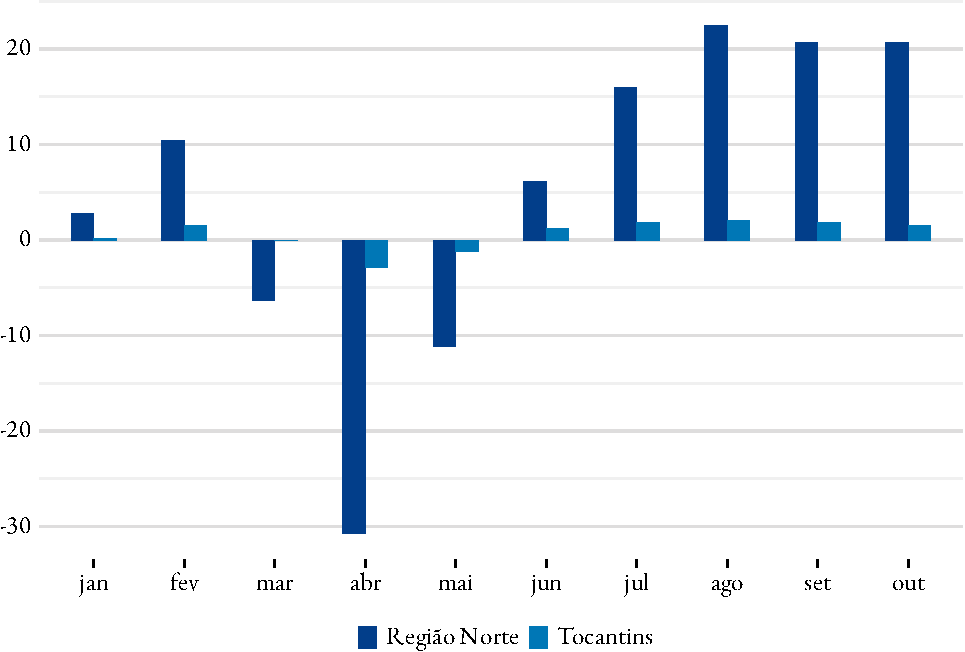
\includegraphics{fig/saldo-1.pdf}

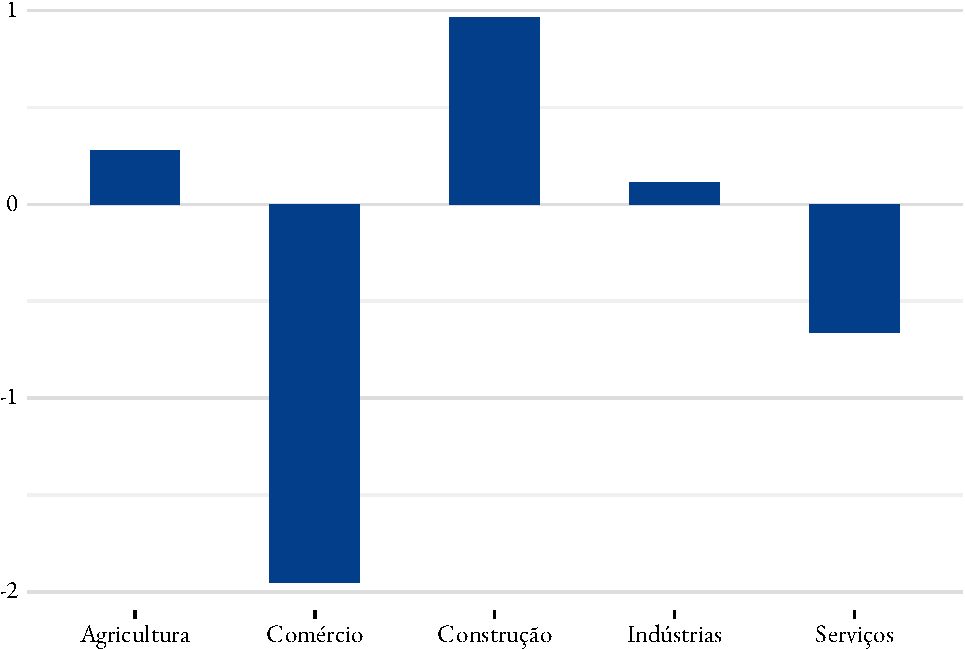
\includegraphics{fig/saldo_setor_to-1.pdf}

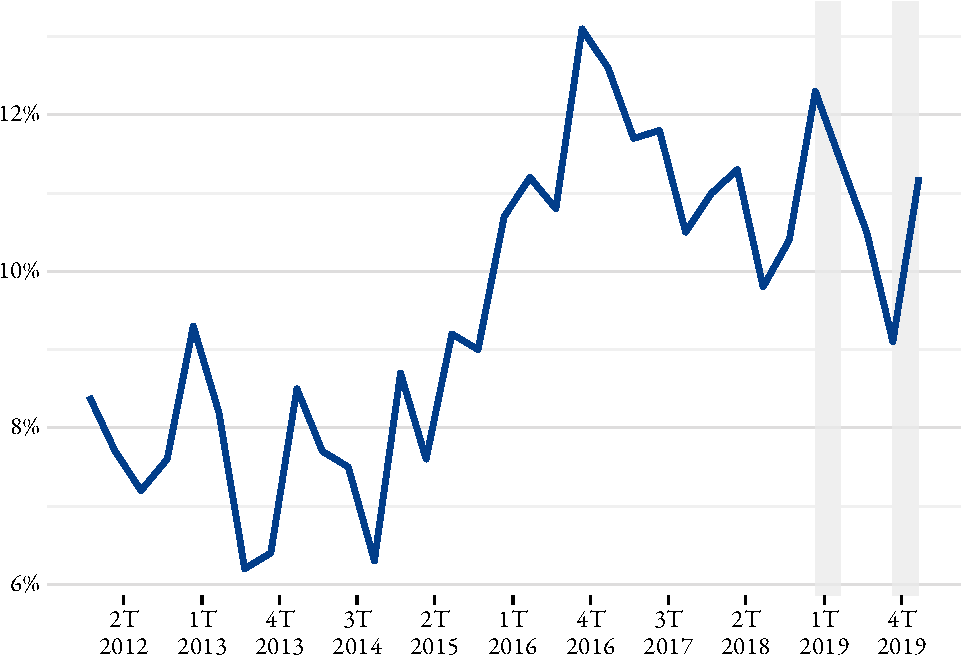
\includegraphics{fig/tx_desemprego_to-1.pdf}

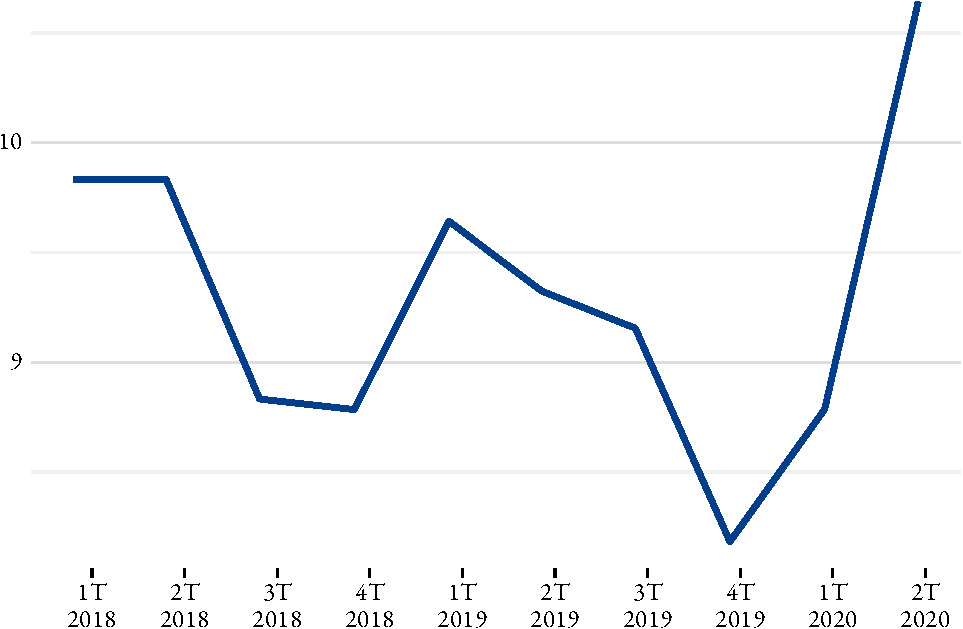
\includegraphics{fig/pedido_segudo_desem-1.pdf}

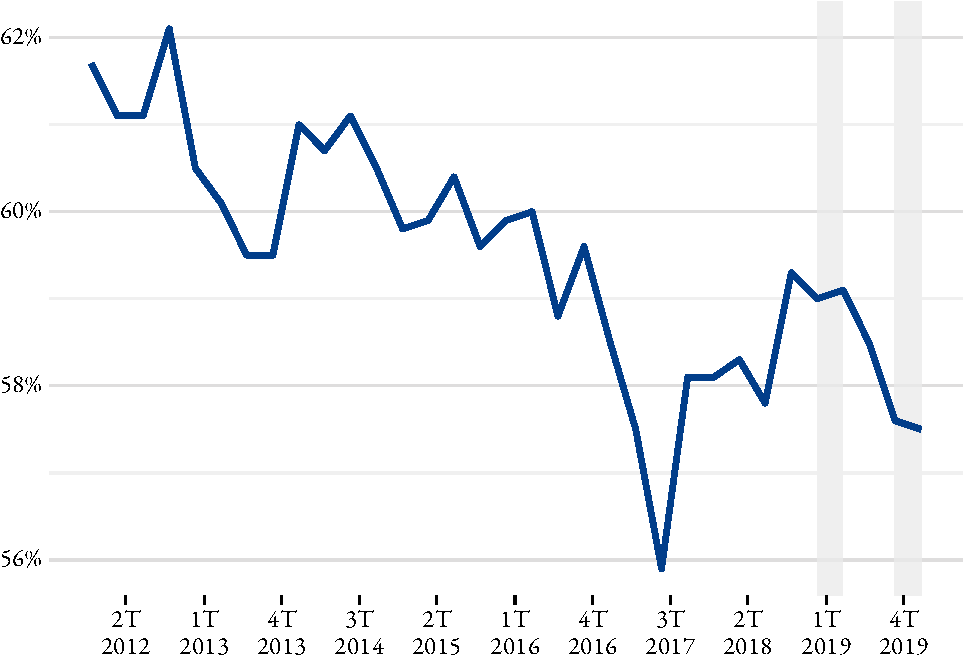
\includegraphics{fig/pop_ocupada-1.pdf}

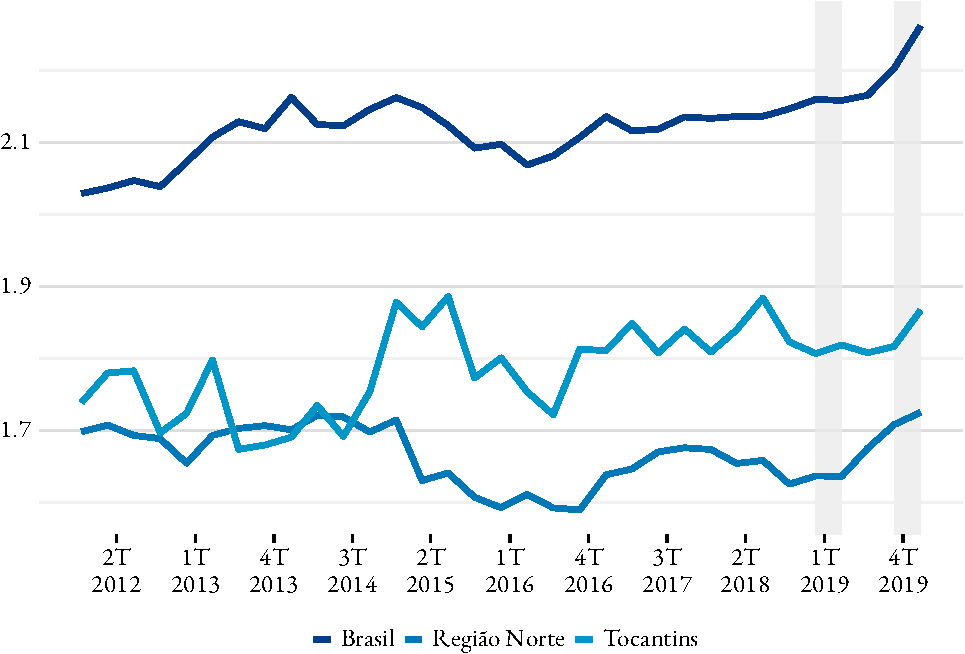
\includegraphics{fig/rend_medio-1.pdf}

\begin{verbatim}
##    (Intercept) taxaDesemprego 
##      3093.4990       566.9133
\end{verbatim}

\begin{verbatim}
## 
## Call:
## lm(formula = Pedidos_SeguroDesemprego ~ taxaDesemprego, data = Dados)
## 
## Residuals:
##     Min      1Q  Median      3Q     Max 
## -657.93 -225.58   19.25  295.72  503.45 
## 
## Coefficients:
##                Estimate Std. Error t value Pr(>|t|)   
## (Intercept)      3093.5     1431.4   2.161  0.06268 . 
## taxaDesemprego    566.9      130.2   4.355  0.00243 **
## ---
## Signif. codes:  0 '***' 0.001 '**' 0.01 '*' 0.05 '.' 0.1 ' ' 1
## 
## Residual standard error: 408.9 on 8 degrees of freedom
## Multiple R-squared:  0.7033, Adjusted R-squared:  0.6662 
## F-statistic: 18.96 on 1 and 8 DF,  p-value: 0.00243
\end{verbatim}

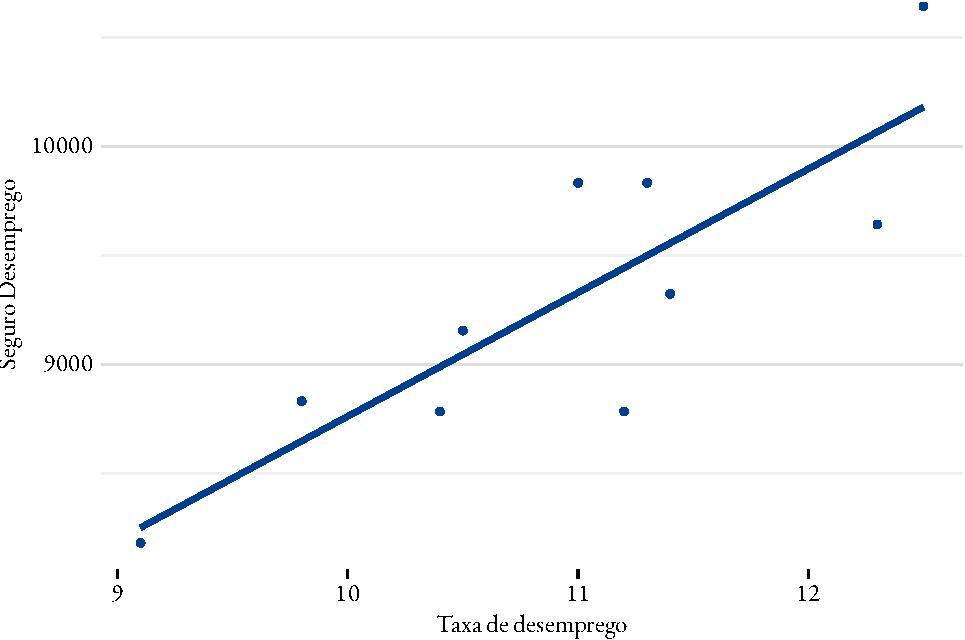
\includegraphics{fig/reg_emprego-1.pdf}

\begin{table}

\caption{\label{tab:unnamed-chunk-1}XXX}
\centering
\begin{tabu} to \linewidth {>{\raggedright}X>{\raggedleft}X>{\raggedleft}X>{\raggedleft}X}
\toprule
 & Admitidos & Demitidos & Saldo\\
\midrule
\addlinespace[0.3em]
\multicolumn{4}{l}{\textbf{Idade}}\\
\hspace{1em}14-34 & 12.933 & 11.375 & 1.558\\
\hspace{1em}35-65 & 5.270 & 5.677 & -407\\
\hspace{1em}65+ & 21 & 59 & -38\\
\addlinespace[0.3em]
\multicolumn{4}{l}{\textbf{Sexo}}\\
\hspace{1em}Homem & 11.043 & 10.869 & 174\\
\hspace{1em}Mulher & 6.243 & 5.736 & 507\\
\bottomrule
\end{tabu}
\end{table}
